\documentclass[11pt]{article}
\usepackage[T1]{fontenc}
\usepackage{lmodern}
\usepackage[margin=1in]{geometry}
\usepackage{amsmath,amssymb}
\usepackage{array}
\usepackage{tabularx}
\usepackage{booktabs}
\usepackage{graphicx}
\usepackage{caption}
\usepackage{subcaption}
\usepackage{tikz}
\usetikzlibrary{arrows.meta,positioning,fit,calc}
\usepackage{url}
\usepackage[hidelinks]{hyperref}
\usepackage[numbers,sort&compress]{natbib}

\captionsetup{font=small,labelfont=bf,margin={2pt,2pt},singlelinecheck=false}
\newcommand{\SI}[2]{#1\,\ensuremath{#2}}
\newcommand{\pp}{\mathrm{pp}}
\newcommand{\percent}{\%}
\setlength{\emergencystretch}{1em}

\title{Pooled Accuracy Is Not Enough to Authorize Fixed-K3 VMD Preprocessing: Same-Source and External Bearing Audits}

\author{Anonymous manuscript for review\\
Affiliation withheld}

\date{}

\begin{document}

\maketitle

\begin{abstract}
\vspace{0.35em}
\noindent
Pooled diagnostic accuracy is widely used to decide whether preprocessing
should be enabled, although measurement condition, validation unit, and class
mix can alter what that number means. We audit this authorization problem using
same-source and external bearing evidence. On HUSTbearing, fixed K3 shows a
clean-trained speed-level gain of \SI{9.72}{\pp}, but matched 0 dB noise
augmentation on both raw and K3 reverses the effect to \SI{-7.94}{\pp}
(unit-only interval [-12.61, -3.44]; crossed robustness interval
[-12.72, -3.28]) and returns Not qualified under the illustrative
$\delta=1$ pp margin. The bearing-level effect is \SI{0.49}{\pp}
[-0.62, 1.53], and bearing-wise pooled balanced accuracy stays below five-class
chance. The speed-minus-bearing contrast of \SI{10.21}{\pp}
[3.67, 19.06] is descriptive across different unit sets, not a paired
per-bearing interaction. In an independent PHM2012 run-to-failure audit with 17
non-fragile bearings, clean-trained K3 raises mean balanced accuracy by
\SI{24.51}{\pp}, but the healthy class rises by \SI{70.75}{\pp} while the
degraded class falls by \SI{-21.73}{\pp} ([-43.14, -5.39]); class safety
therefore fails. Matched augmentation changes the mean effect to
\SI{-6.29}{\pp}. No external block receives a full Qualified status. A
three-state evidence audit distinguishes Not qualified from Insufficient and
organizes the decision, but it is a decision aid, not a validated certification
framework. The empirical contribution is that pooled gains can reverse under
matched measurement conditions and conceal class-specific harm. Raw remains
the conservative default.
\end{abstract}

\noindent\textbf{Keywords:} rolling bearing diagnosis; measurement-conditioned
preprocessing; pooled accuracy; validation unit; class-specific harm;
matched noise augmentation

\section{Introduction}

Bearing faults are a common cause of degradation in rotating machinery, and
vibration diagnosis is most useful when fault evidence can be separated from
competing components \citep{randall2011}. Variational mode decomposition (VMD)
has become a frequent preprocessing choice because it decomposes a
non-stationary signal into a small bank of band-limited modes
\citep{vmd_original}. Studies have applied VMD to rub-impact diagnosis,
wheel-set bearings, incipient faults, locomotive bearings, and noise-robust
diagnosis more generally
\citep{wang2015vmd,li2017independence,dibaj2021incipient,xu2023adaptive,
adaptive_range_vmd}. Reviews of intelligent diagnosis reinforce the same
motivation: better representations can make downstream classification easier
\citep{deep_review}.

The practical question is not whether VMD can improve a carefully selected
example. It is whether a reported gain constitutes sufficient evidence to
enable decomposition for a new measurement. Three research streams are relevant
but do not answer that authorization question. The first optimizes VMD
parameters within one benchmark family
\citep{wang2015vmd,li2017independence,zheng2019dichotomy,jiang2021adaptive,
zhang2018adaptive,xu2023adaptive,ni2022fivmd,song2022selfadaptive}. It finds a
good local decomposition but does not establish whether that decomposition
should be enabled for a different sensor, bearing geometry, load profile, or
class distribution. The second evaluates whether diagnostic representations
remain useful under changing domains and operating conditions
\citep{cross_domain_review,hustbearing_2024}. The third studies data and
evaluation practice, including leakage, benchmark reuse, and optimistic
transfer \citep{vieira2026realistic}. These streams provide methods and
diagnostics, but they do not determine what a reported gain authorizes.

We audit two ways in which that authorization can fail. First, the same HUSTbearing
source is evaluated under a clean-trained baseline and under matched noise
augmentation. A clean-trained speed-level gain of \SI{9.72}{\pp} reverses to
\SI{-7.94}{\pp} once both representations are trained under the same 0 dB
measurement condition. The same-source speed and bearing holdouts also give
different evidence scopes, although their contrast is descriptive rather than a
paired per-bearing interaction. Second, an independent PHM2012 run-to-failure
audit with 17 non-fragile bearings is used as a locked external block. There,
clean-trained K3 improves mean balanced accuracy by \SI{24.51}{\pp}, but the
healthy class improves by \SI{70.75}{\pp} while the degraded class falls by
\SI{-21.73}{\pp}. The apparent pooled gain therefore coincides with
class-specific harm.

The validation unit is the entity held out and generalized over: a motor speed,
a physical bearing, a fault-size group, or a factory case. An evidence block is
a declared family of completed measurements sharing a rig, protocol, or
operating role. The two terms are not interchangeable. Evidence blocks organize
the audit; validation units determine what inference each block can authorize.
A gain observed under an operating-speed holdout does not establish a gain under
physical-bearing holdout, and a clean-versus-noise distinction does not
determine the sign of the downstream effect.

We use a three-state evidence audit to organize the results. Paired unit-level
effect and class-damage intervals are compared with application-defined margins
and mapped to Qualified, Not qualified, or Insufficient. Missing or fragile
class-level evidence returns Insufficient rather than a weaker pass. CCMG is
retained only as an optional measurement-condition prefilter; it is not a
benefit predictor and is not a main contribution.

We address three questions. First, does a clean-trained VMD advantage survive
matched measurement conditions? Second, can a pooled improvement coexist with
class-specific harm under an external target-unit holdout? Third, can a
three-state audit make the difference between demonstrated failure and
insufficient evidence explicit without treating the audit as a validated
certification system?

The contribution is deliberately narrower than a new decomposition algorithm.
It has three parts.

\begin{enumerate}
  \item An empirical falsification of the clean-trained baseline: fixed K3
  changes sign under matched noise augmentation, so the apparent advantage is
  not a sufficient measurement warrant.
  \item An external class-level counterexample: the 17-bearing PHM2012 audit
  shows a large pooled gain together with an entirely negative degraded-class
  interval.
  \item A three-state evidence audit that makes the authorization boundary
  explicit. It is a decision template applied to established intervals, not a
  validated qualification framework.
\end{enumerate}

For measurement practice, the contribution is the empirical demonstration that
pooled accuracy can misauthorize preprocessing and the decision vocabulary that
prevents that result from being read as deployment evidence. The paper does not
propose a new VMD optimizer, classifier, sensor-calibration model, or
uncertainty budget.

\section{Literature Review}

\subsection{VMD parameter selection}

VMD decomposes a non-stationary signal into $K$ band-limited modes through a
variational optimization procedure \citep{vmd_original}. Its use in
rotating-machinery diagnosis has motivated methods for selecting decomposition
parameters and identifying modes that preserve diagnostically useful
information
\citep{wang2015vmd,li2017independence,zheng2019dichotomy,jiang2021adaptive,
zhang2018adaptive,xu2023adaptive,ni2022fivmd,song2022selfadaptive}. These
methods optimize a criterion such as mode independence, envelope concentration,
entropy, or fault-band energy on a development set and report performance on a
test set drawn from the same benchmark family. This design is appropriate for
finding a good local decomposition. It does not establish whether the selected
operation should be enabled for a different sensor, bearing geometry, load
profile, or class distribution. A criterion that ranks candidates under one
protocol need not rank them under another.

\subsection{Cross-domain evaluation and leakage-controlled practice}

A second body of work asks whether diagnostic representations remain useful
under changing domains and operating conditions
\citep{cross_domain_review,hustbearing_2024}. A third studies data and
evaluation practice, including leakage, benchmark reuse, and optimistic
transfer \citep{vieira2026realistic}. Benchmark studies of the CWRU data also
show that file selection, leakage, and evaluation protocol can materially
change reported performance \citep{cwru_dataset,hendriks2022benchmark}. These streams establish that a reported
number can rest on conditions the number itself does not carry. They provide
diagnostics for whether an evaluation is valid; they do not specify what a
valid evaluation authorizes for another declared unit. This distinction matters
because a decomposition can increase spectral concentration while reducing
discriminative information. It can suppress a broadband disturbance, merge
nearby fault components, create correlated mode inputs, or change the relative
difficulty of fault classes. A pooled gain can therefore coexist with
substantial bearing-level reversals.

\subsection{Intervals, equivalence margins, and evidence status}

The individual statistical ingredients used here are established rather than
new. Cross-validated model selection can produce optimistic error estimates
\citep{varma2006bias}, and inference after selection must account for the
selection event \citep{lee2016selective}. Non-inferiority and equivalence
studies formalize materiality and harm margins
\citep{piaggio2006noninferiority}, while clustered or repeated-measure
evaluations require the dependence structure to be respected
\citep{liang1986longitudinal}. These tools provide intervals and tests; they do
not by themselves map validation-unit evidence to a decision. What is missing
is an explicit mapping from paired validation-unit evidence to a decision that
separates authorization, demonstrated failure, and insufficient evidence. A
confidence interval that crosses the materiality margin does not prove failure;
it fails to license release. A missing class-level interval is not a pass; it
is absent evidence.

\subsection{Positioning}

The VMD parameter-selection literature supplies candidate decompositions. The
cross-domain and evaluation-practice literature supplies leakage-aware splits
and transfer diagnostics. The non-inferiority and equivalence literature
supplies intervals and margins. This paper's empirical question is narrower:
when does a reported pooled gain survive a change in measurement condition,
validation unit, or class-level inspection? The three-state audit is used to
organize that question and to prevent an unresolved interval from being read as
a positive result. It is not presented as a new statistical test.

\section{Model, Methodology, and Data}

Table \ref{tab:symbols} summarizes the principal notation used in this
section.

\begin{table}[t]
\centering
\caption{Principal symbols used in Section 3.}
\label{tab:symbols}
\small
\begin{tabularx}{\linewidth}{@{}p{0.18\linewidth}Xl@{}}
\toprule
Symbol & Description & Unit \\
\midrule
$\Delta_u$ & Paired K3-minus-raw balanced-accuracy effect for unit $u$ & pp \\
$[L_u,U_u]$ & Two-sided unit-only interval for $\Delta_u$ & pp \\
$\delta$ & Minimum material benefit & pp \\
$r_{u,c}$ & Paired recall change for class $c$ in unit $u$ & pp \\
$[L_{u,c},U_{u,c}]$ & Simultaneous class-level interval & pp \\
$\eta$ & Maximum tolerated recall loss for any class & pp \\
$s$ & CCMG composite score & dimensionless \\
$\theta$ & CCMG threshold & dimensionless \\
\bottomrule
\end{tabularx}
\end{table}

\subsection{VMD representations and evaluation units}

For a measured window $x(t)$, VMD estimates $K$ modes $u_k(t)$ and center
frequencies $\omega_k$ by solving

\begin{equation}
\min_{\{u_k\},\{\omega_k\}}
\sum_{k=1}^{K}
\left\|
\partial_t\left[
\left(\delta(t)+\frac{j}{\pi t}\right)*u_k(t)
\right]e^{-j\omega_k t}
\right\|_2^2,
\label{eq:vmd}
\end{equation}
subject to $\sum_k u_k=x$. The implementation fixes $\alpha=2000$, $\tau=0$,
and convergence tolerance $10^{-6}$ across all compared representations. These
are analysis constants, not evidence that $\alpha=2000$ is universally optimal.

Raw samples are treated as a one-channel input; the $K$ modes are treated as a
multi-channel input. Within each external dataset, raw and VMD inputs use the
same layer widths, optimizer, learning rate, batch size, and training schedule.
The comparison therefore tests the complete representation pipeline under a
shared training budget, not two capacity-matched encoders. The raw3 capacity
control is post hoc and exploratory; its results are reported in Appendix
Table \ref{tab:raw3-capacity} and should not be interpreted as a
capacity-matched test.

The validation unit is the entity held out and generalized over. Windows,
recordings, and repeated measurements within one unit are not independent
validation units. An evidence block is a declared family of completed
measurements sharing a rig, protocol, or operating role; its validation unit
determines what inference the block can authorize.

\subsection{Matched noise-augmentation protocol}

All external datasets use 2,048-sample, non-overlapping windows normalized
independently by their own mean and standard deviation. The matched
noise-augmentation protocol described below applies specifically to the
same-source HUSTbearing experiment in Sections 4.2 and 4.3. The remaining
external blocks (HSE, HUST-Hanoi, SCA, and Mehran-UET) retain their original
clean-trained evaluation protocols.

For the HUSTbearing experiment, the training/test split is fixed first, and
noise is then added independently to training and test windows.

\paragraph{Raw branch.}
The raw branch receives the clean training windows plus a noisy copy of the
same training windows, as a one-channel input. Test windows receive an
independent noise realization.

\paragraph{K3 branch.}
The K3 branch receives the same clean training windows plus the identical noisy
training copy, decomposed into three modes. Test windows receive the identical
test noise realization used by the raw branch, then decomposed into three
modes.

Both branches therefore share the same raw samples, labels, sample budget,
classifier seed, training schedule, and noise realization. The paired
K3-minus-raw difference is computed on the same held-out unit under the same
noise draw.

\paragraph{Noise-realization structure.}
The matched-augmentation control is identified by the frozen split, training
seed, and a single fixed 0 dB training/test realization set. The crossed
interval resamples training seeds; noise-realization sensitivity is assessed
separately in the clean-trained multi-realization analysis.

\paragraph{Noise-mismatch check.}
To test whether the matched-augmentation result depends on exact training/test
noise matching, both representations are additionally trained at 0 dB and
tested at $-3$ dB and $+4$ dB. These mismatch conditions are robustness checks,
not the primary comparator.

\subsection{PHM2012 external run-to-failure audit}

The external audit uses the complete PHM2012/PRONOSTIA bearing lives
\citep{pronostia2012}. Seventeen bearings are taken from the learning and full
test sets. For each bearing, the first 20\% of its life is labeled healthy and
the last 20\% is labeled degraded; the middle 60\% is excluded. Twelve
acquisitions per class per bearing are sampled at evenly spaced positions inside
each interval. The horizontal acceleration channel is normalized per 2,048
sample window, and the physical bearing is the validation unit in a
leave-one-bearing-out split. The audit uses three classifier seeds and compares
raw with fixed K3 under the same clean-trained and matched-augmentation
protocols. A single fixed 0 dB noise realization is shared by raw and K3; the
result is therefore a locked external audit, not a multi-realization field
study. This endpoint is binary healthy-versus-degraded run-to-failure
classification and is not a reproduction of the five-class HUSTbearing fault
type task.

\subsection{Clean-condition measurement gate}

CCMG is an optional prefilter, not a benefit predictor. For a target rig, let
$m_j$ and $M_j$ be the median and median absolute deviation of feature $j$ in
a clean commissioning baseline. The normalized change is

\begin{equation}
z_j=
\begin{cases}
\dfrac{f_j-m_j}{\max(1.4826M_j,10^{-6})}, & j\in\mathcal{N}_{\uparrow},\\[6pt]
\dfrac{m_j-f_j}{\max(1.4826M_j,10^{-6})}, & j=\mathrm{SNR\ proxy},
\end{cases}
\label{eq:gate-z}
\end{equation}
where $\mathcal{N}_{\uparrow}$ contains spectral flatness, spectral entropy,
high-frequency ratio, envelope entropy, and wavelet noise-to-RMS ratio. The
composite score is

\begin{equation}
s=\frac{1}{|\mathcal{J}|}\sum_{j\in\mathcal{J}} z_j,
\label{eq:gate-score}
\end{equation}
with $\mathcal{J}$ containing the noise-increase features and the SNR proxy.
The threshold $\theta$ is selected only from rigs other than the held-out rig.
Candidate thresholds are quantiles of the training scores, and the objective is
balanced accuracy for clean versus any controlled-noise condition. The
resulting decision answers a narrow measurement question: whether the signal
has moved away from the clean commissioning condition. It does not decide
whether decomposition improves a downstream diagnosis.

\subsection{Three-state evidence audit}

Figure \ref{fig:qualification-flow} summarizes the decision path from a
declared validation unit to the three evidence states. The figure organizes the
audit; it is not presented as a validated decision product.

\begin{figure}[t]
\centering
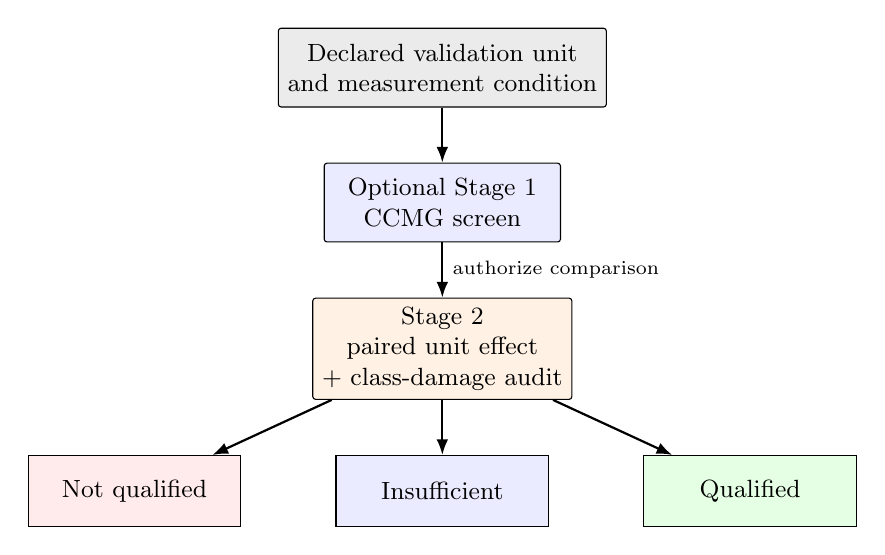
\begin{tikzpicture}[
  node distance=7mm and 9mm,
  box/.style={draw, rounded corners=1pt, align=center, minimum width=30mm,
  minimum height=10mm, font=\small},
  state/.style={draw, align=center, minimum width=27mm, minimum height=9mm,
  font=\small},
  arrow/.style={-{Latex[length=2mm]}, thick}
]
\node[box, fill=black!8] (input) {Declared validation unit\\and measurement condition};
\node[box, below=of input, fill=blue!8] (stage1) {Optional Stage 1\\CCMG screen};
\node[box, below=of stage1, fill=orange!10] (stage2) {Stage 2\\paired unit effect\\+ class-damage audit};
\node[state, below left=of stage2, fill=red!8] (nq) {Not qualified};
\node[state, below=of stage2, fill=blue!8] (ins) {Insufficient};
\node[state, below right=of stage2, fill=green!10] (q) {Qualified};
\draw[arrow] (input) -- (stage1);
\draw[arrow] (stage1) -- node[right, font=\scriptsize]{authorize comparison} (stage2);
\draw[arrow] (stage2) -- (nq);
\draw[arrow] (stage2) -- (ins);
\draw[arrow] (stage2) -- (q);
\end{tikzpicture}
\caption{Three-state evidence audit used in this study. Stage 1 is an optional
measurement-condition screen and may be omitted. Missing or fragile class-level
evidence returns Insufficient. The audit is a decision aid, not a validated
certification framework.}
\label{fig:qualification-flow}
\end{figure}

We distinguish measurement-condition screening from validation-unit evidence
status. For a declared unit $u$, let $\Delta_u$ be the paired
K3-minus-raw balanced-accuracy effect and $[L_u,U_u]$ its two-sided $1-\alpha$
unit-only interval. Let $\delta\geq 0$ be the minimum material benefit and
$\eta\geq 0$ the maximum tolerated recall loss for any class. For class $c$,
let $r_{u,c}$ be the paired recall change and $[L_{u,c},U_{u,c}]$ a
simultaneous interval across classes at the declared confidence level. If
class-level intervals are unavailable, the class-damage condition is treated as
missing, not as satisfied.

The decision template is:

\begin{enumerate}
  \item \textbf{Optional Stage 1: measurement-condition screening.} Compute
  $s$. If $s<\theta$, return raw as default and make no benefit claim. If
  $s\geq\theta$, authorize only a Stage 2 comparison. Stage 1 may be omitted
  when a clean commissioning baseline is unavailable or when
  measurement-condition screening is not required.
  \item \textbf{Stage 2: validation-unit-specific evidence audit.} Estimate
  $[L_u,U_u]$ using paired folds that hold out the declared unit and check the
  worst class-level recall change.
  \item Return \textbf{Qualified} only when $L_u>\delta$, all required class
  intervals are available, valid, and non-fragile, and
  $\min_c L_{u,c}\geq-\eta$. Return \textbf{Not qualified} when
  $U_u\leq\delta$ or $\exists c: U_{u,c}<-\eta$. Otherwise return
  \textbf{Insufficient}.
\end{enumerate}

Class intervals are simultaneous over classes using Bonferroni adjustment at
the declared confidence level. Bonferroni controls family-wise coverage across
classes; it does not stabilize intervals estimated from few independent units.
If a class has too few independent validation units to construct a valid
interval, the evidence is recorded as missing. If the interval can be computed
but rests on two to five independent units, it is marked fragile and does not
by itself license a Qualified decision. If the class-damage interval clearly
exceeds $\eta$ and the interval method is valid, the block can return Not
qualified on class-harm grounds.

The current application is a retrospective worked example; it does not satisfy
the prospective predeclaration condition. The non-fragile requirement is an
audit requirement of this worked example, not a general small-sample
statistical law.

\subsection{Statistics and aggregation}

We report paired percentage-point differences in test accuracy. Three
statistical objects are kept separate:

\begin{center}
\small
\begin{tabularx}{\linewidth}{@{}>{\raggedright\arraybackslash}p{0.23\linewidth}>{\raggedright\arraybackslash}X>{\raggedright\arraybackslash}p{0.27\linewidth}@{}}
\toprule
Object & Statistical meaning & Use \\
\midrule
Unit-only interval & Uncertainty across declared validation units, conditional
on the evaluated protocol & Stage 2 decision interval \\
Crossed interval & Sensitivity to training-seed and, where available,
noise-realization variation & Robustness check \\
Speed-minus-bearing contrast & Descriptive contrast between different held-out
unit sets & Not a paired per-bearing interaction \\
\bottomrule
\end{tabularx}
\end{center}

For the discovery network we fit

\begin{equation}
\Delta_i=\mu+u_{\mathrm{rig}(i)}+v_{\mathrm{protocol}(i)}
+\varepsilon_i,
\label{eq:hierarchical}
\end{equation}
where $u_{\mathrm{rig}}$ and $v_{\mathrm{protocol}}$ are independent mean-zero
random effects.

To audit how conclusions depend on the validation unit, we also analyse 86
heterogeneous paired K3-minus-raw validation units nested in ten evidence
blocks:

\begin{equation}
\Delta_{ij}=\mu+u_i+\varepsilon_{ij},
\label{eq:evidence-block}
\end{equation}
where $i$ indexes evidence blocks and $j$ indexes units within a block. We
report a moment-based variance decomposition, the corresponding intraclass
correlation, and the range of pooled means obtained by leaving out one complete
evidence block. The blocks are not exchangeable independent samples.

For the external physical-bearing audits, a held-out bearing receives all of
its recordings under different speeds or loads. We report the mean and median
paired effect across bearings, a bearing bootstrap interval, and the number of
improved, unchanged, and worsened bearings. Pooled out-of-fold balanced
accuracy is computed from summed confusion matrices and reported descriptively.

For the same-source HUSTbearing split, uncertainty is reported using 20,000
percentile-bootstrap draws. The unit-only interval resamples held-out speeds or
bearings and is the Stage 2 decision interval. The crossed interval
independently resamples held-out units and training seeds, and, where multiple
noise realizations exist, noise realizations. It is reported as a robustness
check.

\section{Results and Discussion}

\subsection{A pooled mean does not define what a validation unit authorizes}

Figure \ref{fig:validation-map} summarizes how the held-out entity determines
the scope of the authorized inference.

\begin{figure}[t]
\centering
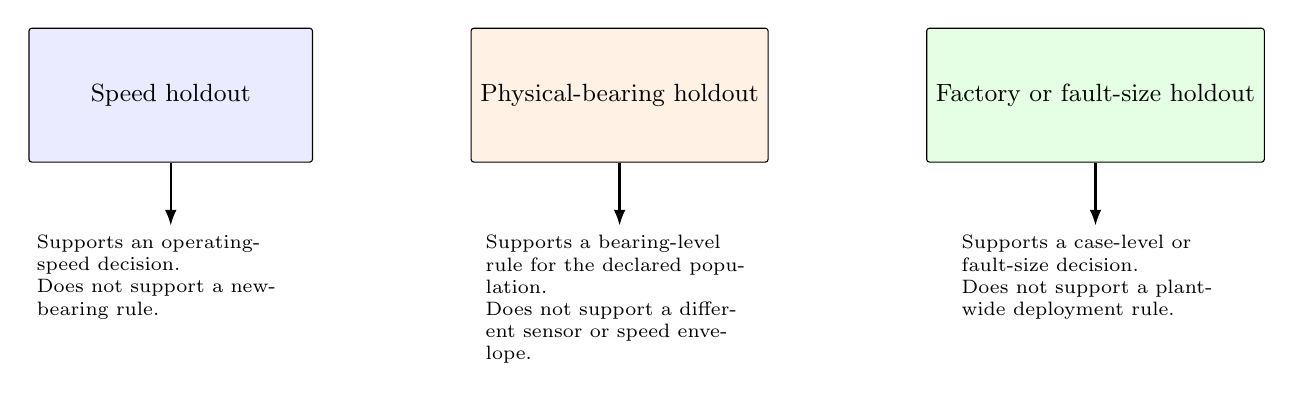
\begin{tikzpicture}[
  node distance=8mm and 20mm,
  block/.style={draw, rounded corners=1pt, align=center, minimum width=36mm,
  minimum height=17mm, font=\small},
  scope/.style={align=left, font=\scriptsize, text width=34mm},
  arrow/.style={-{Latex[length=2mm]}, thick}
]
\node[block, fill=blue!8] (speed) {Speed holdout};
\node[block, right=of speed, fill=orange!10] (bearing) {Physical-bearing holdout};
\node[block, right=of bearing, fill=green!10] (factory) {Factory or fault-size holdout};
\node[scope, below=of speed] (speed-text) {Supports an operating-speed decision.\\Does not support a new-bearing rule.};
\node[scope, below=of bearing] (bearing-text) {Supports a bearing-level rule for the declared population.\\Does not support a different sensor or speed envelope.};
\node[scope, below=of factory] (factory-text) {Supports a case-level or fault-size decision.\\Does not support a plant-wide deployment rule.};
\draw[arrow] (speed) -- (speed-text);
\draw[arrow] (bearing) -- (bearing-text);
\draw[arrow] (factory) -- (factory-text);
\end{tikzpicture}
\caption{Validation units and the scope of inference. The held-out entity
determines what a completed evaluation can authorize.}
\label{fig:validation-map}
\end{figure}

\begin{table}[t]
\centering
\caption{Validation units and evidence boundaries. Mean effects are relative to
clean-trained raw. The rows are evidence blocks, not exchangeable independent
samples. The HUSTbearing value is the original speed-holdout run; Table
\ref{tab:same-source} reports the separate same-source fixed-budget rerun.}
\label{tab:validation-units}
\scriptsize
\begin{tabularx}{\textwidth}{@{}>{\raggedright\arraybackslash}p{0.11\textwidth}>{\raggedright\arraybackslash}p{0.09\textwidth}>{\raggedright\arraybackslash}p{0.13\textwidth}rrr>{\raggedright\arraybackslash}X>{\raggedright\arraybackslash}X@{}}
\toprule
Evidence block & Role & Unit & $n$ & Mean $\Delta$ (pp) & Signs (+/0/$-$) & Supports & Does not support \\
\midrule
CWRU & discovery rig & condition/file fold & 1 & +6.00 & 1/0/0 & Controlled noise sensitivity & Cross-bearing transfer \\
JNU & discovery rig & condition fold & 1 & +25.50 & 1/0/0 & Severe-noise sensitivity & Evidence-block-wide rule \\
MFPT & discovery rig & rig protocol & 1 & +44.00 & 1/0/0 & Independent-rig response & Bearing-level generalization \\
Ottawa & discovery condition & condition fold & 4 & +0.59 & 2/0/2 & Condition-wise reversals & Stable clean/noise boundary \\
Paderborn & discovery protocol & protocol fold & 3 & -0.31 & 1/0/2 & Protocol sensitivity & Transferable mode-count rule \\
HUSTbearing & speed holdout & motor speed & 10 & +7.61 & 8/0/2 & Operational speed holdout & Physical-bearing transfer \\
HSE & bearing holdout & physical bearing & 11 & +10.81 & 6/3/2 & Leave-one-bearing-out test & Stable positive block effect \\
HUST-Hanoi & bearing holdout & physical bearing & 33 & -0.42 & 11/17/5 & Leave-one-bearing-out test & General K3 benefit \\
SCA & industrial holdout & factory case & 10 & -4.11 & 5/0/5 & Case-level transfer audit & Factory-wide deployment \\
Mehran-UET & fault-size holdout & fault-size group & 12 & -11.81 & 5/1/6 & Decision-boundary audit & Fault-physics mechanism \\
\bottomrule
\end{tabularx}
\end{table}

A pooled mean across 86 heterogeneous validation units in ten evidence blocks
is \SI{0.88}{\pp}. Read in isolation, that positive value suggests that K3
helps. Table \ref{tab:validation-units} shows why the pooled value is not an
authorization: the block means reverse in sign, and leaving out one complete
evidence block moves the pooled mean between \SI{-0.58}{\pp} and
\SI{2.93}{\pp}. The same treatment can be positive for one block and negative
for another because the blocks answer different questions. A motor-speed fold
asks whether an operating-speed decision transfers. A physical-bearing fold
asks whether the decision survives when the bearing itself changes. A
fault-size fold asks how the class boundary responds. These are not
interchangeable samples from one evidence block.

Read row by row, the table separates four kinds of authorization. CWRU, JNU,
and MFPT establish controlled or rig-level sensitivity, not transfer to new
bearings. Ottawa and Paderborn show that protocol composition can reverse the
direction inside the discovery panel. HUSTbearing provides a clean-trained
speed-level comparator, but the matched-augmentation audit does not authorize
an operational decision. HSE, HUST-Hanoi, SCA, and Mehran-UET test four
different physical or industrial units; their signs do not form one
exchangeable sample.

The moment-based between-block standard deviation is \SI{10.53}{\pp} and the
within-block standard deviation is \SI{32.59}{\pp}; the resulting ICC is 0.095.
A maximum-likelihood fit places the between-block component near zero. These
estimates do not support a claim that between-block variance dominates. They do
not, however, make the validation unit irrelevant. Small between-block variance
can coexist with sign reversals at the level of the declared unit, and block
composition still changes the direction and scope of the pooled conclusion.

\subsection{Same-source split: speed-wise versus bearing-wise}

\begin{figure}[t]
\centering
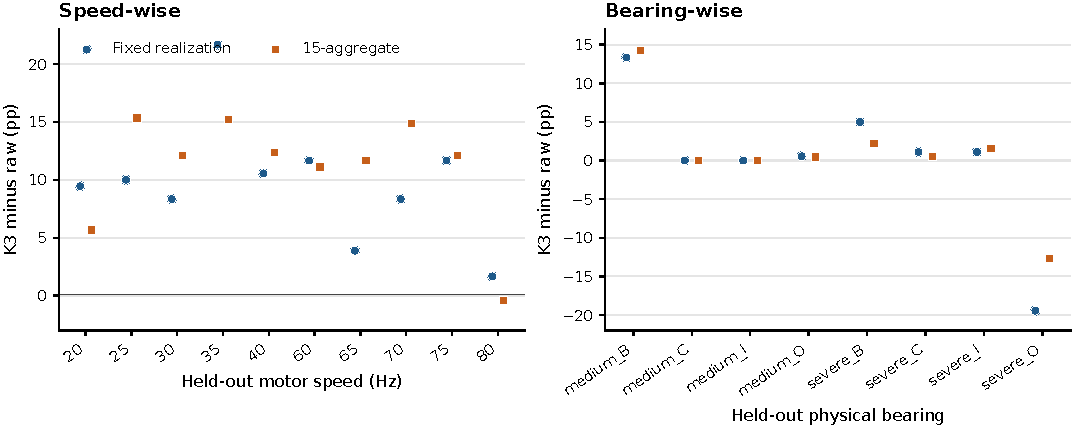
\includegraphics[width=0.96\linewidth]{figures/final_same_source_split.pdf}
\caption{Same-source HUSTbearing split under the original realization and the
15 seed/noise aggregate. Each point is a held-out validation unit. The
speed-level gain and bearing-level neutrality describe different estimands.}
\label{fig:same-source}
\end{figure}

\begin{table}[t]
\centering
\caption{Same-source HUSTbearing split comparison and noise-realization
sensitivity. Fixed rows use the original realization. The multi-realization
rows aggregate three seeds and five noise realizations. Unit-only intervals
are the Stage 2 decision intervals; crossed intervals are robustness checks.}
\label{tab:same-source}
\scriptsize
\begin{tabular}{@{}llrrrrrr@{}}
\toprule
Scheme & Realization & Units & Mean $\Delta$ & Unit-only 95\% CI & Crossed 95\% CI & Signs & Raw/K3 BA \\
\midrule
Speed & fixed & 10 & +9.72 & [6.83, 13.00] & -- & 10/0/0 & 22.44/32.17 \\
Speed & 15 aggregate & 10 & +11.00 & [7.88, 13.51] & [6.72, 15.10] & 9/0/1 & 22.94/33.94 \\
Bearing & fixed & 8 & +0.21 & [-6.39, 5.56] & -- & 5/2/1 & 3.40/3.61 \\
Bearing & 15 aggregate & 8 & +0.79 & [-4.22, 5.78] & [-6.68, 5.72] & 5/2/1 & 2.90/3.69 \\
\bottomrule
\end{tabular}
\end{table}

Figure \ref{fig:same-source} and Table \ref{tab:same-source} report the
decisive same-source HUSTbearing split. The analysis holds the data
source fixed while changing the validation-unit set. The unit-only interval is
computed by aggregating the prespecified training seeds and noise realizations
within each held-out unit, then resampling the independent held-out units. The
15 seed-by-noise aggregates are repeated experimental combinations, not 15
independent validation units. The single-realization speed-wise estimate is
\SI{9.72}{\pp} with unit-only interval [6.83, 13.00]. The 15-aggregate
speed-wise estimate is \SI{11.00}{\pp} with unit-only interval
[7.88, 13.51] and crossed interval [6.72, 15.10]. The bearing-wise estimates
are \SI{0.21}{\pp} (single realization, unit-only [-6.39, 5.56]) and
\SI{0.79}{\pp} (15 aggregate, unit-only [-4.22, 5.78], crossed
[-6.68, 5.72]). The speed-minus-bearing contrast is \SI{10.21}{\pp}
(crossed interval [3.67, 19.06]) and corresponds to the 15-aggregate
estimates; the single-realization contrast is \SI{9.51}{\pp}. The contrast
also changes training-bearing coverage: a speed holdout leaves recordings from
the test bearing at other speeds in training, whereas a bearing holdout removes
the test bearing entirely. It therefore compares different validation-unit
sets and training coverage and is not a paired per-bearing interaction.

The absolute pooled balanced accuracies also require interpretation. Speed-wise
pooled out-of-fold balanced accuracy is \SI{22.44}{\percent} for raw and
\SI{32.17}{\percent} for K3. Bearing-wise pooled out-of-fold balanced accuracy
is \SI{3.40}{\percent} and \SI{3.61}{\percent} under clean training, and
\SI{1.32}{\percent} and \SI{1.81}{\percent} under matched augmentation, for a
five-class problem whose uniform-random reference is \SI{20}{\percent}
(Table \ref{tab:bearing-ba}). The class-supported analysis excludes bearings
whose training partition lacks at least one class; the eight retained bearings
cover all five classes. Each physical bearing contributes one class, so the
bearing-level value is a class-recall comparison, not a complete multi-class
diagnostic capability estimate.

\begin{table}[t]
\centering
\caption{Bearing-wise pooled out-of-fold balanced accuracy for the same eight
class-supported bearings. BA = $(1/5)\sum_c \mathrm{Recall}_c$. The 20\%
five-class uniform-random level is a reference baseline, not an operational
capability threshold.}
\label{tab:bearing-ba}
\footnotesize
\begin{tabular}{@{}llrr@{}}
\toprule
Training protocol & Validation scope & Raw BA & K3 BA \\
\midrule
Clean-trained & Bearing-wise, 8 supported bearings & 3.40\% & 3.61\% \\
Matched augmentation & Bearing-wise, same 8 supported bearings & 1.32\% & 1.81\% \\
\bottomrule
\end{tabular}
\end{table}

\subsection{Matched noise augmentation reverses the clean-trained advantage}

\begin{figure}[t]
\centering
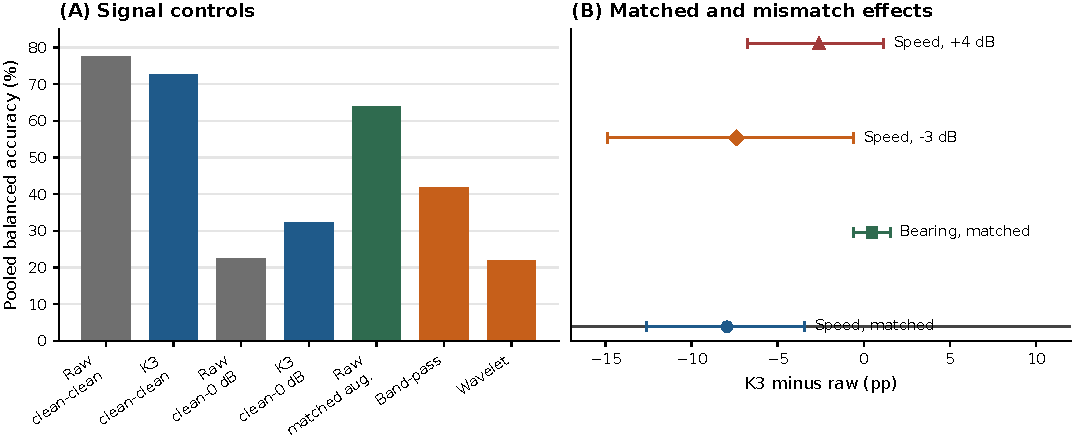
\includegraphics[width=0.96\linewidth]{figures/final_matched_augmentation.pdf}
\caption{Matched-augmentation and signal controls on HUSTbearing. (A) Pooled
balanced accuracy for clean, noise-augmented, band-pass, and wavelet
conditions. (B) Paired K3-minus-raw effects with unit-only intervals.}
\label{fig:matched-augmentation}
\end{figure}

\begin{table}[t]
\centering
\caption{HUSTbearing matched-augmentation and noise-mismatch control. Unit-only
intervals are decision intervals; crossed intervals in the text are robustness
checks. The bearing analysis excludes the healthy bearing.}
\label{tab:matched-augmentation}
\scriptsize
\begin{tabular}{@{}llrrrrrr@{}}
\toprule
Scheme & Test condition & Units & Mean $\Delta$ & Unit-only 95\% CI & Crossed 95\% CI & Signs & Raw/K3 BA \\
\midrule
Speed & matched 0 dB & 10 & -7.94 & [-12.61, -3.44] & [-12.72, -3.28] & 2/1/7 & 63.83/55.89 \\
Bearing & matched 0 dB & 8 & +0.49 & [-0.62, 1.53] & [-0.83, 1.67] & 4/3/1 & 1.32/1.81 \\
Speed & train 0, test -3 dB & 10 & -7.39 & [-14.89, -0.61] & -- & 3/0/7 & 54.67/47.28 \\
Speed & train 0, test +4 dB & 10 & -2.61 & [-6.78, 1.17] & -- & 4/1/5 & 65.94/63.33 \\
Bearing & train 0, test -3 dB & 8 & -0.83 & [-2.08, 0.21] & -- & 2/2/4 & 2.92/2.08 \\
Bearing & train 0, test +4 dB & 8 & +0.42 & [-0.42, 1.67] & -- & 1/6/1 & 0.28/0.69 \\
\bottomrule
\end{tabular}
\end{table}

Figure \ref{fig:matched-augmentation} and Table
\ref{tab:matched-augmentation} report the matched-augmentation and signal
controls. The clean-trained comparison is deliberately vulnerable: clean-to-clean
controls work (raw 77.56\%, K3 72.56\%), but clean-to-0 dB performance collapses
(raw 22.44\%, K3 32.17\%). Noise-augmented raw reaches 63.83\%, while
band-pass and wavelet controls reach 41.83\% and 22.00\%. The clean-to-0 dB
degradation is consistent with substantial train/test measurement shift. The
band-pass and wavelet controls are trained on clean windows and tested at
0 dB; they are descriptive signal-processing controls, not
matched-augmentation competitors.

When raw and K3 are both trained on clean windows plus the same noisy training
realization, speed-wise raw reaches 63.83\% and augmented K3 reaches 55.89\%;
the paired K3-minus-raw effect is \SI{-7.94}{\pp} (unit-only decision interval
[-12.61, -3.44]; crossed robustness interval [-12.72, -3.28]), with seven of
ten speeds negative. At the bearing level, the corresponding pooled
out-of-fold balanced accuracies are 1.32\% and 1.81\%, with a mean difference
of \SI{0.49}{\pp} (unit-only interval [-0.62, 1.53]; crossed interval
[-0.83, 1.67]). The clean-trained K3 advantage over a vulnerable raw baseline
therefore does not survive matched noise augmentation.

The sign change is not an artifact of exact training/test noise matching. When
both representations are trained at 0 dB and tested at $-3$ dB, the speed-wise
effect is \SI{-7.39}{\pp} (unit-only interval [-14.89, -0.61]); at $+4$ dB it
is \SI{-2.61}{\pp} ([-6.78, 1.17]). At $-3$ dB, the estimated effect remains
negative and its interval excludes zero. At $+4$ dB, the point estimate is
also negative, but the interval crosses zero. These mismatch conditions are
robustness checks, not the primary comparator.

\subsection{External evidence: pooled gain with class-specific harm}

\begin{figure}[t]
\centering
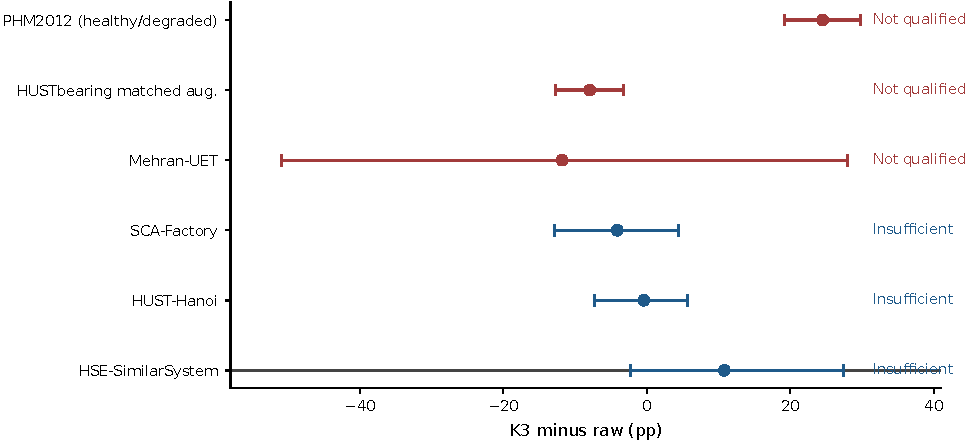
\includegraphics[width=0.88\linewidth]{figures/final_external_forest.pdf}
\caption{Evidence states for the PHM2012 run-to-failure block,
the external fault-type blocks, and the matched-augmentation HUSTbearing
comparison. Intervals are unit-only decision intervals.}
\label{fig:external-forest}
\end{figure}

\begin{table}[t]
\centering
\caption{Worked evidence states under the illustrative margins
$\delta=1$ pp and $\eta=5$ pp. The PHM2012 rows use a separate
run-to-failure healthy/degraded endpoint with 17 independent bearings. All
intervals shown are unit-only decision intervals; crossed robustness intervals
are reported in the text.}
\label{tab:qualification-states}
\footnotesize
\begin{tabularx}{\linewidth}{@{}lrrlX@{}}
\toprule
Block & Units & Mean $\Delta$ (pp) & Unit-only 95\% CI & Status / basis \\
\midrule
PHM2012 clean-trained (H/D) & 17 & +24.51 & [19.20, 29.74] & Not qualified / class harm \\
PHM2012 matched (H/D) & 17 & -6.29 & [-12.17, -0.98] & Not qualified / mean effect \\
HSE & 11 & +10.81 & [-2.31, 27.44] & Insufficient / mean and class inconclusive \\
HUST-Hanoi & 33 & -0.42 & [-7.32, 5.72] & Insufficient / mean and class inconclusive \\
SCA & 10 & -4.11 & [-12.89, 4.40] & Insufficient / mean and class inconclusive \\
Mehran-UET & 12 & -11.81 & [-50.93, 28.01] & Not qualified / class harm \\
HUSTbearing matched aug. & 10 & -7.94 & [-12.61, -3.44] & Not qualified / mean effect \\
HUSTbearing matched bearing & 8 & +0.49 & [-0.62, 1.53] & Insufficient / mean interval crosses zero \\
\bottomrule
\end{tabularx}
\par\smallskip
\parbox{\linewidth}{\footnotesize HUSTbearing crossed robustness interval:
[-12.72, -3.28]. It is not the decision interval.}
\end{table}

Figure \ref{fig:external-forest} and Table
\ref{tab:qualification-states} compare the PHM2012 external audit, the four
blocks with saved class-level confusion matrices, and the primary
matched-augmentation HUSTbearing speed comparison using the same interval
audit.
The PHM2012 clean-trained row is the clearest class-level failure: the mean
effect is \SI{24.51}{\pp} with lower bound \SI{19.20}{\pp}, but the healthy
class changes by \SI{70.75}{\pp} [57.52, 83.66] while the degraded class
changes by \SI{-21.73}{\pp} [-43.14, -5.39]. The degraded upper bound is below
the illustrative \SI{-5}{\pp} harm margin, so the block is \textbf{Not
qualified} despite its positive pooled mean. Under matched augmentation, the
PHM2012 mean effect falls to \SI{-6.29}{\pp} [-12.17, -0.98] and is Not
qualified on the mean-effect branch.

With matched augmentation as the primary HUSTbearing baseline, the speed-level
effect is \SI{-7.94}{\pp} with unit-only interval [-12.61, -3.44]. Because the
unit-only upper bound, \SI{-3.44}{\pp}, is below $\delta=1$ pp, the K3 decision
is \textbf{Not qualified}. The crossed interval [-12.72, -3.28] is a robustness
check, not the decision interval.

The matched bearing-level effect is \SI{0.49}{\pp} [-0.62, 1.53]. Its interval
crosses zero, so the bearing-level result is \textbf{Insufficient}, not neutral
and not a deployment rule.

HSE, HUST-Hanoi, and SCA remain Insufficient because their mean-effect
intervals cross zero and their class intervals do not establish that harm is
within the allowed margin. Mehran-UET is Not qualified: although its mean
interval crosses zero, strong inner-class damage beyond the example harm margin
is present. Class intervals for HSE and HUST-Hanoi are based on only 2--5 units
with positive support for each class, so they are marked fragile. No block is
promoted to Qualified. The full class support, paired recall change,
simultaneous interval, fragile flag, missing flag, and harm decision are
reported in Appendix Table \ref{tab:qualification-class-audit}.

\subsection{What the result means}

The results support three claims in order of evidence strength. First, a
pooled gain is not stable under measurement condition. The HUSTbearing
clean-trained speed-level gain of \SI{9.72}{\pp} reverses to
\SI{-7.94}{\pp} when raw and K3 receive matched noise augmentation. The
clean-trained gain is therefore a baseline-specific observation, not a
preprocessing warrant.

Second, a positive pooled gain can conceal class-specific harm. In PHM2012,
the clean-trained mean effect is \SI{24.51}{\pp}, but the degraded-class
interval is [-43.14, -5.39] and fails the harm margin. This is stronger
evidence than a generic warning about heterogeneity: the aggregate metric and
the class-level decision point in opposite directions.

Third, a validation-unit holdout changes the scope of the claim. The
speed-minus-bearing contrast is descriptive and is not a paired per-bearing
interaction, so it cannot establish a causal interaction. It does show that a
speed-level result cannot be used as a physical-bearing rule without a
separate bearing-level audit. The three-state evidence audit makes these
statuses explicit, but the empirical conclusion rests on the reversal and the
class-specific harm, not on the labels themselves. CCMG remains an optional
screen with limited incremental value.

\section{Conclusion and Future Work}

\subsection{Conclusion}

This study shows that pooled diagnostic accuracy is not sufficient to authorize
VMD preprocessing. Two empirical results carry the argument. First, on the same
HUSTbearing source, a clean-trained speed-level gain of \SI{9.72}{\pp} reverses
to \SI{-7.94}{\pp} (unit-only interval [-12.61, -3.44]; crossed robustness
interval [-12.72, -3.28]) once both raw and K3 are trained with matched 0 dB
augmentation. Second, in the independent PHM2012 run-to-failure audit with 17
non-fragile bearings, clean-trained K3 raises mean balanced accuracy by
\SI{24.51}{\pp}, but the healthy class gains \SI{70.75}{\pp} while the degraded
class loses \SI{21.73}{\pp}. The pooled gain therefore coexists with an
entirely negative degraded-class interval, and the block is Not qualified on
class-harm grounds. Matched augmentation changes the PHM2012 mean effect to
\SI{-6.29}{\pp}.

No external block receives a full Qualified label. The matched-augmentation
HUSTbearing speed audit is Not qualified under the illustrative $\delta=1$ pp
margin; its bearing-level result is unresolved; HSE, HUST-Hanoi, and SCA remain
Insufficient; Mehran-UET is Not qualified due to inner-class harm; PHM2012 is
Not qualified under both its clean-trained and matched protocols. The
three-state audit makes these evidence statuses explicit, but it is an audit
template rather than a validated certification system. CCMG remains an optional
prefilter with small incremental value.

The paper does not establish a universal K3 rule, a benefit predictor, or a
deployment recommendation. It establishes that pooled accuracy can misauthorize
preprocessing when measurement conditions, validation units, or class-specific
effects are not included in the decision. Raw remains the conservative default.

\subsection{Future work}

Matched noise augmentation should be repeated across the remaining external
blocks and across multiple noise realizations in PHM2012. PHM2012 uses a
different binary healthy/degraded endpoint and a single fixed noise
realization, so its result should not be read as a five-class replication or a
field validation. HSE, HUST-Hanoi, and SCA remain Insufficient under their
clean-trained protocols, whereas Mehran-UET is Not qualified under the
illustrative class-damage margin.

Class-complete validation units are also needed. HSE and HUST-Hanoi have
positive class support in only 2--5 units, which makes their class-level
intervals fragile and prevents a full Qualified decision. A prospective
target-unit study should pre-specify power or precision before fixing the number
of validation units; the synthetic boundary case in Appendix Figure
\ref{fig:operating} shows that ten units yield only about 15\% Qualified under
borderline benefit, so ten units are not a default minimum sample size.

The clean-baseline features are signal-quality indicators, not calibrated
sensor uncertainties. A measurement-chain study that records sensor type,
mounting, sampling rate, and maintenance state would make the CCMG threshold
more transportable. A fault-physics mechanism analysis would require trusted
shaft speed and bearing geometry, which the present evidence does not provide.
Until such evidence exists, the three-state audit should be read as a decision
aid for declared validation units, not as a universal deployment rule.

\section*{Data and Code Availability}

The analysis code, frozen protocols, generated tables, figures, and result
files accompany the submission. Source datasets retain their original licenses
and access conditions. The reproducibility artifact is available at
\url{https://github.com/KKK-cell441/fixed-k3-pooled-accuracy-audit}.

\section*{Ethics Declaration}

Not applicable. This study uses previously collected bearing vibration
datasets and does not involve human participants, animals, or personally
identifiable information.

\section*{CRediT Author Contributions}

The authors jointly designed the study, curated the datasets, implemented the
analysis, interpreted the results, and wrote the manuscript.

\section*{Conflict of Interest}

The authors declare no conflict of interest.

\section*{Funding}

This research received no specific grant from any funding agency in the
public, commercial, or not-for-profit sectors.

\section*{AI Disclosure}

AI-assisted tools were used for analysis scripting, manuscript drafting, and
internal consistency checks. All numerical results were generated from the
documented analysis artifacts. The authors have verified the numerical outputs
against the artifacts.

\clearpage
\appendix
\setcounter{figure}{0}
\renewcommand{\thefigure}{A\arabic{figure}}
\setcounter{table}{0}
\renewcommand{\thetable}{A\arabic{table}}

\section{Additional controls}

\subsection{CCMG ablation}

Figure \ref{fig:ccmg} shows the ablation result.

\begin{figure}[t]
\centering
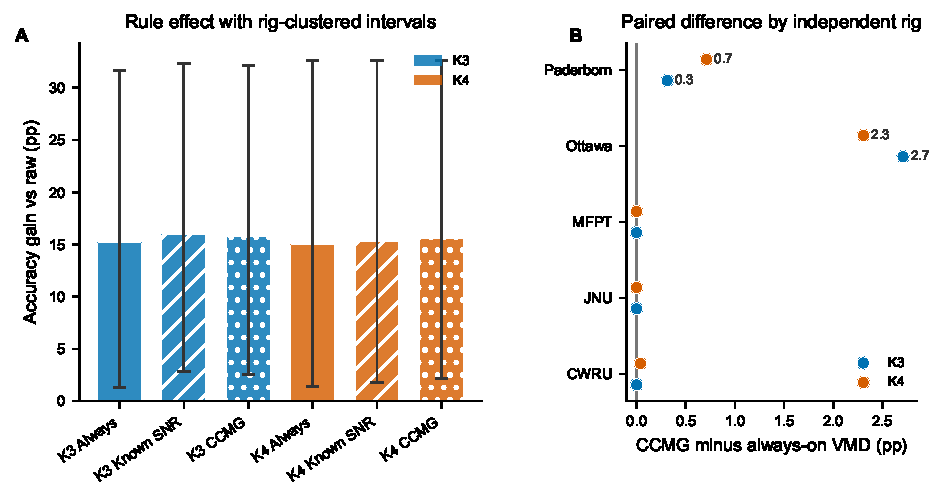
\includegraphics[width=0.95\linewidth]{figures/ccmg_policy_comparison.pdf}
\caption{CCMG ablation. The optional gate changes only a small number of
comparisons and does not predict downstream K3 benefit.}
\label{fig:ccmg}
\end{figure}

The CCMG screen avoided 2 of 86 comparisons and changed the
evidence-block-equalized selected effect by 0.30 pp. Its perfect clean/noise
separation in the controlled grid does not establish field-noise recognition
or diagnostic-benefit prediction.

\subsection{Decomposition-family comparison}

Figure \ref{fig:decomposition-family} reports the protocol-conditional
comparison.

\begin{figure}[t]
\centering
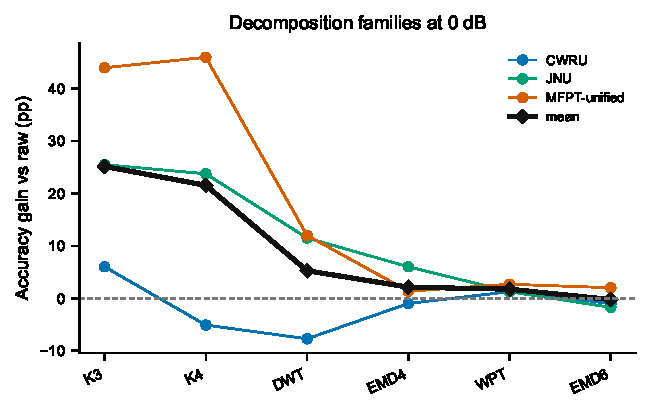
\includegraphics[width=0.95\linewidth]{figures/decomposition_family_comparison.pdf}
\caption{Protocol-conditional decomposition-family comparison. The comparison
is relative to the vulnerable clean-trained raw baseline and does not establish
a general VMD advantage.}
\label{fig:decomposition-family}
\end{figure}

\subsection{Nested mode selection}

Figure \ref{fig:nested-k} and Table \ref{tab:run-level} summarize the nested
selection and run-level audit.

\begin{figure}[t]
\centering
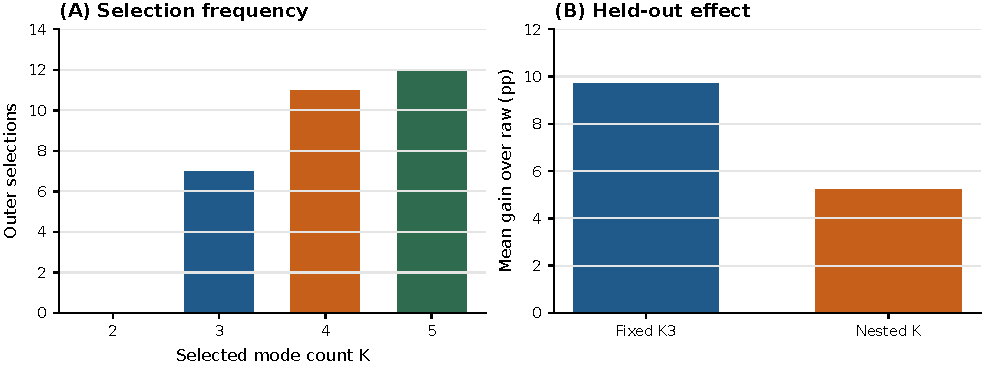
\includegraphics[width=0.92\linewidth]{figures/final_nested_k.pdf}
\caption{Nested K selection on HUSTbearing. Inner validation selects K3 in only
7 of 30 outer-fold/seed selections; fixed K3 is a controlled comparator, not a
selected policy.}
\label{fig:nested-k}
\end{figure}

\begin{table}[t]
\centering
\caption{raw3 capacity control and evidence-block summary. The control repeats
the one-channel raw window three times and is exploratory.}
\label{tab:raw3-capacity}
\scriptsize
\begin{tabular}{@{}llrrr@{}}
\toprule
Block & Unit & $n$ & K3--raw (pp) & K3--raw3 (pp) \\
\midrule
CWRU & condition/file fold & 1 & +6.00 & -- \\
JNU & condition fold & 1 & +25.50 & -- \\
MFPT & rig protocol & 1 & +44.00 & -- \\
Ottawa & condition fold & 4 & +0.59 & -- \\
Paderborn & protocol fold & 3 & -0.31 & -- \\
HUSTbearing & motor speed & 10 & +7.61 & +7.22 \\
HSE & physical bearing & 11 & +10.81 & +10.45 \\
HUST-Hanoi & physical bearing & 33 & -0.42 & -0.34 \\
SCA & factory case & 10 & -4.11 & -4.46 \\
Mehran-UET & fault-size group & 12 & -11.81 & -12.04 \\
\bottomrule
\end{tabular}
\end{table}

\begin{table}[t]
\centering
\caption{Run-level audit summary. Repeat counts describe repeated experimental
combinations, not additional independent validation units.}
\label{tab:run-level}
\footnotesize
\begin{tabularx}{\linewidth}{@{}>{\raggedright\arraybackslash}p{0.22\linewidth}>{\raggedright\arraybackslash}p{0.16\linewidth}rrrX@{}}
\toprule
Block & Validation unit & Units & Seeds & Noise realizations & Protocol role \\
\midrule
HUSTbearing, speed, clean-trained & motor speed & 10 & 3 & 5 & noise-realization sensitivity \\
HUSTbearing, speed, matched & motor speed & 10 & 3 & 1 & primary matched audit \\
HUSTbearing, bearing, clean-trained & physical bearing & 8 & 3 & 5 & same-source sensitivity \\
HUSTbearing, bearing, matched & physical bearing & 8 & 3 & 1 & same-source matched audit \\
HSE & physical bearing & 11 & 2 & 1 & external bearing audit \\
HUST-Hanoi & physical bearing & 33 & 2 & 1 & external bearing audit \\
SCA & factory case & 10 & 2 & 1 & industrial audit \\
Mehran-UET & fault-size group & 12 & 2 & 1 & industrial audit \\
PHM2012 clean & run-to-failure bearing & 17 & 3 & 1 & locked external audit \\
PHM2012 matched & run-to-failure bearing & 17 & 3 & 1 & locked external audit \\
\bottomrule
\end{tabularx}
\end{table}

\section{Operating characteristics and field actions}

Figure \ref{fig:operating} reports the synthetic operating characteristics,
and Table \ref{tab:field-actions} maps each state to a field action.

\begin{figure}[t]
\centering
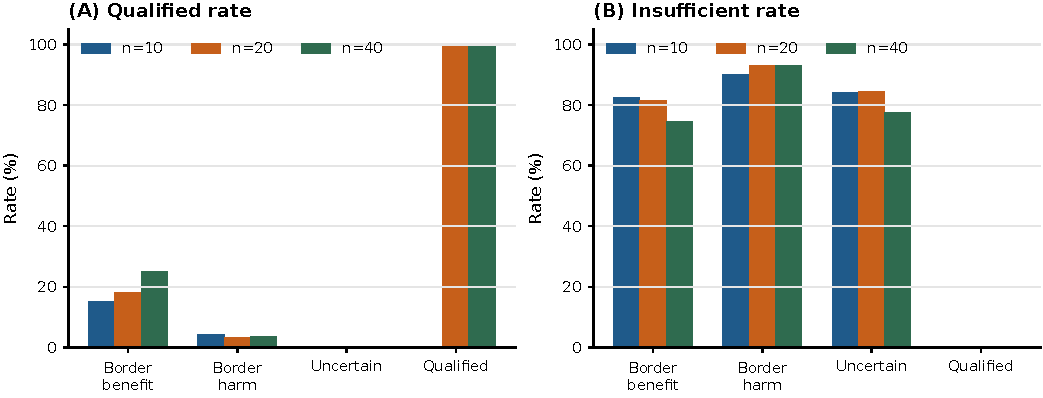
\includegraphics[width=0.95\linewidth]{figures/final_operating_characteristics.pdf}
\caption{Synthetic operating characteristics of the three-state rule under
independent validation units and Gaussian class-level changes. The simulation
is not an empirical coverage calibration.}
\label{fig:operating}
\end{figure}

The boundary-benefit scenario yields Qualified rates of roughly 15--25\% and
mostly Insufficient. The boundary-harm scenario produces roughly 3--4\% false
Qualified decisions. These results depend on the stated simulation assumptions
and do not establish coverage under the dependence structure of the observed
datasets.

\begin{table}[t]
\centering
\caption{Field actions for the three authorization states.}
\label{tab:field-actions}
\small
\begin{tabularx}{\linewidth}{@{}>{\raggedright\arraybackslash}p{0.14\linewidth}>{\raggedright\arraybackslash}X>{\raggedright\arraybackslash}X@{}}
\toprule
State & Immediate action & Required follow-up \\
\midrule
Qualified & Enable the candidate only for the declared validation unit and
operating envelope; log the version and margins. & Monitor drift and re-qualify
after any change in sensor, mounting, speed/load, bearing type, fault mix, or
baseline condition. \\
Not qualified & Keep raw as the production default; do not enable the
candidate for that unit. & Reopen only with a new prespecified comparator,
unit, or measurement condition; do not reinterpret the same test outcome as a
qualified result. \\
Insufficient & Keep raw or use a controlled engineering pilot without a
production benefit claim. & Add independent units, missing class support, or
the missing class-level interval; then repeat Stage 2. Do not resolve
insufficiency by weakening $\delta$, $\eta$, or the confidence level. \\
\bottomrule
\end{tabularx}
\end{table}

\section{Class-level evidence audit}

\input{qualification_class_audit_table.tex}

The table exposes the evidence behind each worked evidence state. The
decision column is evaluated against the same illustrative harm margin used in
the main text. Missing or inconclusive class evidence is not converted into a
pass. Mehran-UET has strong evidence of inner-class harm and no comparable
evidence of outer-class harm, whereas HSE and HUST-Hanoi have several
inconclusive classes because their bearing-level folds do not contain every
class in every validation unit.

\section{Benefit-predictor audit}

Figure \ref{fig:benefit-audit} reports the evidence-block benefit-predictor
audit.

\begin{figure}[t]
\centering
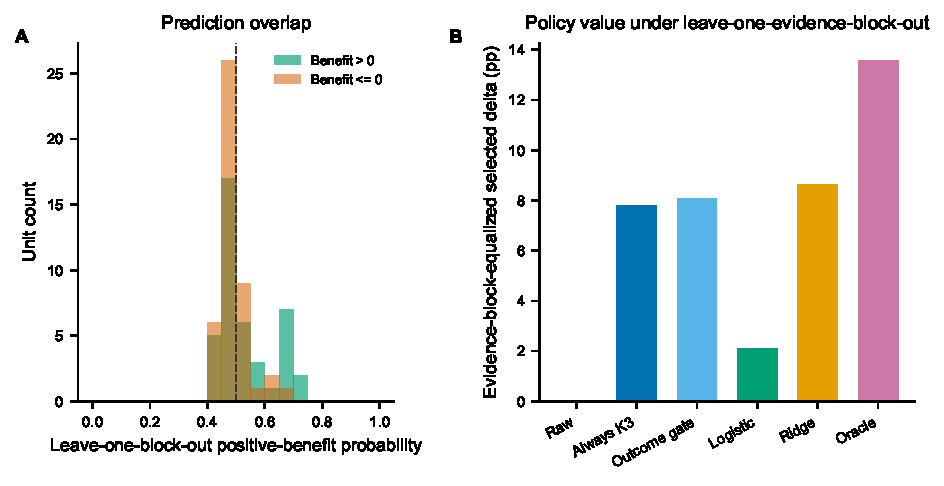
\includegraphics[width=0.95\linewidth]{figures/benefit_predictor_audit.pdf}
\caption{Evidence-block benefit-predictor audit. The four-feature models do not
support a reliable cross-block selection rule.}
\label{fig:benefit-audit}
\end{figure}

The four-feature logistic model reached AUROC 0.651 and the ridge model reached
AUROC 0.514. The blind-noise feature alone reached AUROC 0.687. The ridge point
estimate is \SI{8.64}{\pp}, slightly above the \SI{7.79}{\pp} all-K3 value in
the policy audit, but its near-chance discrimination and mean absolute error of
\SI{22.4}{\pp} do not support a reliable selector interpretation.

\section{Reproducibility and limitations}

This is a secondary analysis of completed measurements and classifier runs.
All severe-noise results use additive white Gaussian noise, not a field-noise
campaign. The discovery synthesis combines completed classifier runs from
several protocols. The external audits share layer widths, optimizer, learning
rate, batch size, and training budget, but K3 has three input channels and
therefore 576 additional first-layer parameters. The comparison is not a pure
VMD-representation effect isolated from every architecture difference.

HUST-Hanoi and HSE each contain a finite number of physical bearings, and
several operating conditions belong to the same bearing. The exact mode count
remains protocol dependent. K3 was fixed before the external audits but was not
selected on an independent validation partition within the discovery data.
The other external blocks still use fixed test realizations and clean-trained
raw. The crossed bootstrap treats the finite seed and noise levels as
resampling factors, so its interval is a sensitivity interval rather than a
large-sample guarantee. The synthetic simulation is not an empirical coverage
calibration.

The evidence blocks are interpreted as separate worked audits rather than as
one prespecified family of hypothesis tests; no global multiplicity-corrected
claim is made. Leave-one-speed folds share most of their training data, so the
unit bootstrap quantifies variation across held-out speeds, not independent
training replication. The HUST-Hanoi normal class has an interval
[-62.22, -2.22] that excludes zero but does not cross the illustrative
$-5$ pp harm margin; the rule therefore returns Insufficient, separating
evidence of decline from evidence of unacceptable harm. An exploratory
fixed-candidate audit over K2--K5 on HUSTbearing also returned no Qualified
status; clean-trained K5 was closest, with mean \SI{4.72}{\pp} [2.56, 6.78]
and an outer-class interval [-11.94, 6.39]. K4/K5 were not carried into the
PHM2012 matched-augmentation audit. PHM2012 uses one fixed noise realization
and a binary run-to-failure endpoint, so its result is a locked external
audit, not a five-class replication or field validation.

All numerical tables are generated from saved CSV or JSON artifacts. The
analysis manifest records hashes for source summaries, scripts, figures, and
reports. No result was filtered by outcome direction. The neutral HUST-Hanoi
result, the negative HUSTbearing fold, the negative SCA and Mehran-UET means,
and the negative HSE bearings are retained.

\bibliographystyle{unsrtnat}
\bibliography{references}

\end{document}
